 \documentclass{sig-alternate}
\usepackage{graphicx}
\usepackage{subfigure}
\usepackage{stmaryrd}

% PASSW for PEPM: pe06stups

\newcommand{\logen}[2]{$\underbrace{\texttt{#2}}_{{\footnotesize #1}}$}
\newcommand{\unfold}[1]{\logen{unfold}{#1}}
\newcommand{\memo}[1]{\logen{memo}{#1}}

% Standard Definitions

\newcommand{\NN}{\mbox{${I\!\!N}$}}
\newcommand{\RR}{\mbox{${I\!\!R}$}}
\newcommand{\ZZ}{\mbox{${Z\!\!\!Z}$}}

\def\mymath#1{\relax\ifmmode#1\else$#1$\fi}
\newcommand{\sembra}[2]{\mymath{[\![#1]\!]_{\rm#2}}}
\newcommand{\sem}[1]{\mymath{[\![#1]\!]}}

\newcommand{\theoremstart}[2]{{\bf #1 #2}}
\newcommand{\theoend}{\hspace*{\fill}\(\Box\)}

\newcounter{defcounter}[section]
\renewcommand{\thedefcounter}{\thesection.\arabic{defcounter}}

\newenvironment{algorithm}%
{\refstepcounter{defcounter} \begin{trivlist} \item[]%
\theoremstart{Algorithm}{\thedefcounter}}%
{\end{trivlist}}

\newenvironment{zitemize}% zero - line spacing itemize environment
   {\begin{list}{--}{
   \setlength{\itemsep}{0 pt}
   \setlength{\parsep}{0 pt}
   \setlength{\topsep} {0 pt} }}% the end stuff
   {\end{list}}
\newenvironment{pitemize}% zero - line spacing itemize environment for programs
   {\begin{list}{}{
   \setlength{\itemsep}{0 pt}
   \setlength{\parsep}{0 pt}
   \setlength{\topsep} {2 pt} }}% the end stuff
   {\end{list}}
\newcommand{\mikearraystretch}{1}
\newcommand{\var}[1]{#1}
\newcommand{\svar}[1]{\mbox{{\scriptsize #1}}}

\newcommand{\larr}{\leftarrow}


\newcommand{\diff}{\mathit{\backslash\!==}}
\newcommand{\dif}{\mathit{\backslash\!=}}

\newcommand{\MSG}[2]{\mathit{msg}(#1,#2)}
\newcommand{\MGU}[1]{\mathit{mgu}(#1)}


\newcommand{\homeo}{\unlhd}
\newcommand{\nothomeo}{\not\!\unlhd}
\newcommand{\homeostrict}{\lhd}


\newcommand{\ignore}[1]{} % {{\tt \small ignore(#1)}}
\newcommand{\forExperts}[1]{} % {{\small {\bf For Experts Only:}\\ #1}}
\newcommand{\comment}[1]{}



\numberofauthors{2}
\title{The Logen System and Web Interface}
\author{
\alignauthor Michael Leuschel \& Stephen-John Craig\\
       \affaddr{University of D\"{u}sseldorf, Germany}\\
       \email{leuschel@cs.uni-duesseldorf.de}
       % ORDER TO BE DETERMINED
\alignauthor Daniel Elphick\thanks{The authors have been partially
supported by the Information Society
Technologies programme of the European Commission, Future and Emerging
Technologies under the IST-2001-38059 ASAP project.}\\
       \affaddr{University of Southampton, United Kingdom}\\
       \email{dre@ecs.soton.ac.uk}
}
\CopyrightYear{2005}

\pagestyle{plain} %empty,plain

\begin{document}


\maketitle

\begin{abstract}
We present the {\sc logen} partial evaluation system, a new implementation in Ciao Prolog with
fully stand-alone generating extensions, as well as a sophisticated Web
Interface.
\end{abstract}


% ----------------------------------------------
\section{The Logen System}

Partial evaluation \cite{Jones:peval}
 is a well known program specialisation technique.
 Partial evaluators can be broadly classified into
 online and offline systems.
An offline system works in two phases:
 the first phase produces an annotated version of the source program.
These annotations steer the second phase: the partial evaluation
phase proper.
Given a self-applicable offline partial evaluator,
 one can construct a so-called {\em
  compiler generator\/} (a {\em cogen\/} for short) 
  using Futamura's third projection (see e.g. \cite{Jones:peval}).
 A {\em cogen} is a program that given an annotated source
  program produces a specialiser for that program.
If the source program is an interpreter, this specialiser can be
viewed as a compiler, hence the name ``compiler generator.''
However, obtaining an efficient cogen by self-application is a quite difficult task.
This has led several researchers to pursue
 the so-called {\em cogen approach}
to program specialisation
\cite{Holst:89a,HolstLaunchbury:92,%
BirkedalWelinder:94:handcogen,Andersen94:PhD,GlueckJoergensen:PLILP95,%
Thiemann:ICFP96}.
The idea behind this approach is to write
 the {\em cogen\/}  directly by hand, rather than trying to obtain it by
 self-application.
The application of the cogen approach in a logic programming setting
has led to the {\sc logen} system
\cite{JorgensenLeuschel:Cogen,LeuschelEtAl:TPLP03}.
Figure~\ref{figure:logen} highlights the way the {\sc logen} system works.
Typically, a user would proceed as follows:

  
\begin{figure}[htb]
\begin{center}
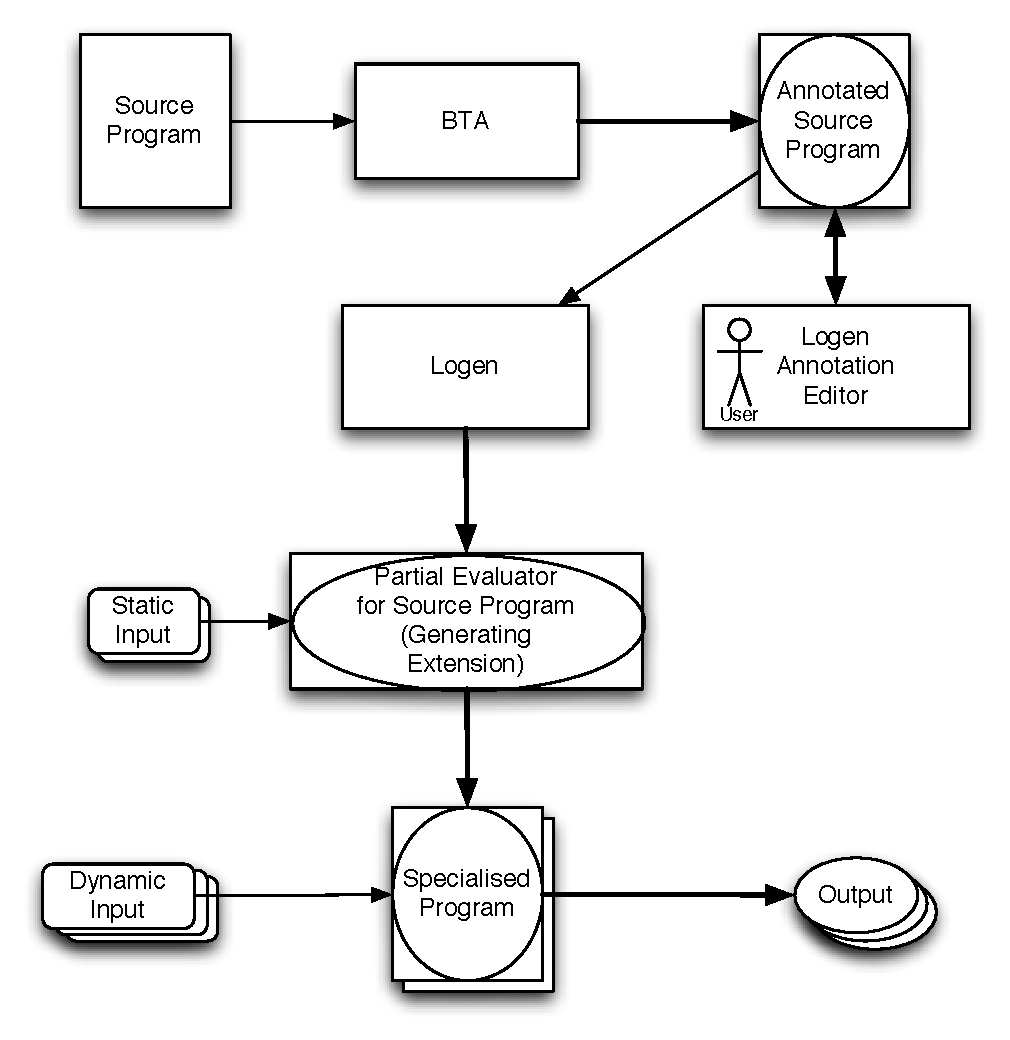
\includegraphics[width=3.5in]{logen}
\end{center}
\caption{Illustrating the {\sc logen} system and the $\mathit{cogen}$ approach}
\protect\label{figure:logen}
\end{figure}




\begin{zitemize}
\item First the source program is annotated using the binding-time analysis
 (BTA), which
  produces an annotated source program.  This annotated source program
  can be further edited, which
  allows an expert to inspect and manually refine the annotations
  to get better specialisation. 
  
\item Second, {\sc logen} is run on the annotated source program and
  produces a specialiser for the source program, called a {\em
    generating extension}.
   
\item This generating extension can now be used to specialise the
  source program for some static input. Note that the same generating
  extension can be run many times for different static inputs (i.e.,
  there is no need to re-run {\sc logen} on the annotated source
  program unless the annotated source program itself changes).
    
\item As soon as the remainder of the input is known, the specialised
  program can be run and will produce the same output as the
  original source program.  Note again, that the same specialised
  program can be run for different dynamic inputs;  the specialised program 
  only has to be regenerated if the static input changes (or
  the original program itself changes).
 \end{zitemize}


The particularities of the {\sc logen} system are:
 \begin{zitemize}
 \item Efficient specialisation through the use of specialised specialisers.
\item Support for partially static data, with user-definable binding-types. For example,
 the following defines  a list of variable bindings, with statically 
 known variable names but unknown (at specialisation time) variable values:
 
 \begin{footnotesize}
\begin{verbatim}
 :- type env ---> [] ;
         [ bind(static,dynamic) | type(env)].
\end{verbatim}
  \end{footnotesize}
  
\item Support for almost full Prolog, e.g., the if-then-else, negation,
  disjunction, findall, the cut, built-ins, modules, 
   higher-order calls,...
  
\item An automatic BTA   \cite{BTA:Lopstr04} which ensures termination of the unfolding process.
 The BTA uses the binary clause semantics to identify potential infinite loops in the
  specialised specialiser.
  In addition,  {\sc logen} contains two simple BTAs which annotate
 everything as static and unfold/call or dynamic and memo/rescall respectively.
These can be used in circumstances where the automatic BTA cannot be
 used, e.g., in cases where the source program is large and the automatic BTA
 is too expensive.
The automatic BTA can also be used just to propagate the static/dynamic information
 without trying to infer terminating clause annotations. 
  
\item A watchdog mode which detects non-terminating annotations 
 as well as support for online unfold annotations and online binding-type 
\cite{LeuschelCraig:SemiWatch}, using online control techniques
 such as the homeomorphic embedding relation.

\item An extension for Constraint Logic Programming  has been
 presented in \cite{CraigLeuschel:PSI03}, while support for co-routining
  ({\tt when} declarations)  has
  also been developed \cite{Craig:Phd}.
\item A self-tuning resource aware specialisation method
  that adapts the annotations for a particular architecture and
 set of representative sample queries \cite{CraigLeuschel:PPDP05}.
 \end{zitemize}

\section{Applications}

Various experimental evaluations of the {\sc logen} system
 have been reported, see for example \cite{LeuschelEtAl:TPLP03}.
In essence, specialisation without the binding-time analysis
  turns out to be very fast (several orders of magnitude faster than
 online specialisers). 
 The quality of the specialisation of course depends highly on
 the annotation, but the experiments show that with the proper annotations 
 specialisation can be on par with online specialisers.

{\sc logen} has been applied to numerous interpreters
 and \cite{Leuschel:lopstrbook} contains a systematic study on
  how to apply {\sc logen} to interpreters in general, and how to
 achieve ``Jones optimality'' in particular.

In  \cite{BarkerLeuschelVarea:pepm04}
 {\sc logen} has been succesfully applied to
 a flexible meta-interpreter for %performing
access control checks
on deductive data\-bases.
By specialisation of this interpreter one obtains
  flexible access control with virtually zero overhead.


In \cite{WangGuptaLeuschel:PADL05}
{\sc logen} has been used towards the goal of provably correct compilation
 by specialising denotational semantics language specifications expressed in Horn logic
  and definite clause grammars.
In particular, the semantics for the SCR specification language was
 expressed, and {\sc logen} generated target code in a provably correct manner.
 
 {\sc logen} has also been used as a preprocessor to achieve efficient model checking
  for domain specific specification languages.
For example, in \cite{LeuschelMassart:LOPSTR99} a CTL model checker was specialised for
  particular systems and specific temporal logic formulas.
 In \cite{LeuschelLehmann:Coverability,LeuschelLehmann:CL2000}
  {\sc logen} was used to precompile a Petri net interpreter for later infinite model
   checking.
  In 
  \cite{FarwerLeuschel:PPDP04} an interpreter for Object Petri nets was specialised
  together with the CTL model checker to achieve efficient verification.
{\sc logen} is also currently being applied to improve the efficiency
 of the expressive pointcut language for
 aspect-orientation from \cite{Ostermann:ECOOP05}.
Finally in the ASAP project (EU FET IST-2001-38059) 
 {\sc logen} was used to
 specialise an emulator (written by Kim Henriksen and John Gallagher)
 for the machine language of PIC processors, for analysis purposes.

%[Mention \cite{MartinLeuschel:PSI99} ?]

\section{Re-implementation in Ciao}

The very first version of {\sc logen} \cite{JorgensenLeuschel:Cogen} was
 implemented in BIM Prolog. {\sc logen} was then ported to
   SICStus Prolog.
Within the ASAP EU project  {\sc logen} was re-implemented in
 Ciao Prolog.
 One motivation was the integration with the {\sc ciaopp} program
  analysis toolset and support for platforms with limited resources.
From a pragmatic point of view, the
{\tt ciaoc} compiler allows to easily create stand-alone executables, which made
it very easy to develop a freely distributable command-line version of {\sc logen}.
Furthermore, the fact that Ciao Prolog allows including the compiler
 in runtime systems%
\footnote{Academic licenses of SICStus Prolog do not allow the distribution
 of the Prolog compiler in packaged runtime systems.
Unfortunately, the
 automatic BTA still requires SICStus Prolog since we do not have 
 a robust convex hull solver in Ciao Prolog yet.
This is packaged up as a separate binary, which does not require access to
 the Prolog compiler.}
enables a user to produce generating extensions which are fully stand-alone,
without any further need for the  {\sc logen}
  system.
 Indeed, this is one of the cited advantages of the {\sc cogen} approach, which has thus
 come true.



\section{The Web Interface}

Previous versions of {\sc logen} had various graphical front ends,
 implemented in Tcl/Tk, XEmacs, and Python/Tk respectively.
Distribution and installation of these front ends was not always unproblematic,
and we have now moved to a more elegant web interface, providing a user-friendly interface
for running {\sc logen} and editing the annotations.
A main advantage of the web interface over the earlier interfaces is its portability and
 the ability to run {\sc logen} remotely
  without local installation (even though we also cater for local execution).
  
  
%can be tried out at  the address:\\
%  {\small\tt http://stups.cs.uni-duesseldorf.de/\~{}pe/weblogen}.

The web interface
provides a way to annotate programs and then specialise them. 
Colour coding is used to provide visual feedback about the annotations
 (e.g., static parts are marked green, dynamic parts red).
 The web interface also ensures that the source file and
 the annotation file are kept in sync: if the user changes the source file the changes
  will be detected and only the changed parts have to be re-annotated.
  
{\bf Security:}
Security was an important aspect in the design process of the web interface,
 as allowing untrusted users access to a {\sc logen} system installed on a web server 
 opens up security holes: in particular we need to prevent the execution of unsafe
  Prolog code
  submitted by users (e.g., {\tt\small system('rm *.*')}).
When the web interface invokes {\sc logen}, it thus requests a
\emph{safe} generating extension. Whenever this generating extension tries to
\emph{call} a Prolog predicate, it is first checked against a whitelist of safe
predicates. Arities are listed along with names as some predicates are safe
with one number of arguments, but not with another. Trying to call an unsafe predicate
will cause the process to abort and warn the user.

Our whitelist also allows use of the \texttt{call} predicate and solution
aggregation predicates such as \texttt{findall} and \texttt{bagof}, but only
if the predicate argument is itself in the whitelist.

Besides arbitrary code execution, the interface also has to handle accidental
or deliberate denial of service (DOS) attacks due to infinite unfolding or
memoization. Spawned processes are automatically killed when a time limit is
exceeded, but currently there is a risk that too many simultaneous
connections could overload the server and cause even legitimate processes to
time out without completing.

The interface can also be used on a local machine so long as it has a web
server. With this usage safe mode can be disabled, although it is advised
to restrict access to trusted users only through server mechanisms. The 
specialisation time-out can also be extended in the case of more cpu-intensive
code.

{\bf Displaying and Editing Annotations:}
The annotation system maintains two files: a source file (Figure
\ref{figure:append} shows append) and an annotation file (Figure
\ref{figure:append}). Our interface preserves the formatting of the source code
and overlays the annotations using colours and underlining to distinguish the
different types. Converting the source and annotation file to HTML is a
two-stage process shown in Figure \ref{figure:ann2html}. First an XML
representation (Figure \ref{figure:append_xml}) is created using a Prolog program that matches the annotations
to the source code. This process keeps the structure and comments from the
original source code. The XML is then processed by an XSL transform which
creates HTML code containing style sheet information and Javascript hooks as shown
in Figure \ref{figure:append_html}. Having
two stages simplifies each stage and allows a separation of skills, where a
Prolog programmer can create simple structured XML in the first stage, while
web programmers can control the second without intimate knowledge of Prolog.

\begin{figure}[htb]
\begin{center}

\includegraphics[width=3.5in]{ann2html}
\end{center}
\caption{Converting source and annotation files to HTML}
\protect\label{figure:ann2html}
\end{figure}

\begin{figure}[htb]
\begin{verbatim}
append([],Y,Y).
append([X|Xs],Y,[X|Zs]) :-
    append(Xs,Y,Zs).
\end{verbatim}
\caption{Prolog source for \texttt{append.pl}}
\protect\label{figure:append}
\end{figure}

\begin{figure}[htb]
\begin{verbatim}
logen(append/3,append([],A,A)).
logen(append/3,append([B|C],A,[B|D])) :-
    logen(memo,append(C,A,D)).
:- filter
    append(dynamic,dynamic,dynamic).
\end{verbatim}
\caption{Annotation file for \texttt{append.pl}}
\protect\label{figure:append_ann}
\end{figure}

\begin{figure}[htb]
\begin{verbatim}
<?xml version="1.0" encoding="UTF-8"?>
<article>
<source><head>append</head>([],Y,Y).
<head>append</head>([X|Xs],Y,[X|Zs]) :-
    <memo>append</memo>(Xs,Y,Zs).

</source>
<filters>
:- filter
    <filter>append</filter>(dynamic,dynamic,dynamic).
</filters>
</article>
\end{verbatim}
\caption{XML produced by annotation reader. (Some tags used only for syntax
highlighting have been removed to aid clarity)}
\protect\label{figure:append_xml}
\end{figure}

\begin{figure}[htb]
\begin{verbatim}
<pre class="source">
<span class="head">append</span>([],Y,Y).
<span class="head">append</span>([X|Xs],Y,[X|Zs]) :-
    <span class="memo" id="ann16"
       onclick="return dropdownmenu(this, event)"
       onmouseover="mouseoverAnn('ann16')"
       onmouseout="mouseoutAnn('ann16')"
    >append</span>(Xs,Y,Zs).
</pre>

...

<pre>
:- filter
    <span class="filter">append</span>(dynamic,
                                       dynamic,
                                       dynamic).
</pre>
\end{verbatim}
\caption{HTML produced from \texttt{append.pl}}
\protect\label{figure:append_html}
\end{figure}
Javascript is used extensively so that programs can be annotated without
repeated loading of new pages from the server. Instead clicking on an annotated
predicate brings up a menu of possible annotations and selecting one changes the
HTML code locally on the server; the changes are only sent to the server when the
user has finished. The annotations are sent to the server as a flat list of the 
form:
\begin{verbatim}
[unfold, unfold, memo, call]
\end{verbatim}

These annotations are then mapped back onto the source using a Prolog
executable, \texttt{annotate}, resulting in an annotated program. Since the
filters are more free-form, they are edited and sent back as text from the
client (even though a limited form of editing, such as changing static arguments to dynamic or vice-versa
 can be performed directly using the mouse).
 The server passes this text to \texttt{annotate}, which parses and
appends the result to the annotation file.

\section{Conclusion}

%It is of course difficult to produce a commercial quality tool in an academic
% environment, but since

Since  the appearance of the
   first version of {\sc logen} in 1996 in \cite{JorgensenLeuschel:Cogen}
  the system has now achieved a certain maturity, has been applied
  to numerous case studies and is now in a state where it can be used
  by programmers who are not researchers in partial evaluation.
Indeed, the first version of {\sc logen} was efficient, but
 only supported a small subset of
 Prolog and all annotations had to be performed by hand.
{\sc logen} now supports almost full Prolog, provides a command-line
 interface, has considerable support
for annotating source code
and especially the web interface has lowered the entry threshold for
 using the system.
We hope that the {\sc logen} system will thus prove to be valuable
 to researchers and programmers alike.

\bibliographystyle{abbrv}
\bibliography{michael}

\newpage

\appendix

\section{Command-Line Options}
 \begin{footnotesize}
\begin{verbatim}
Usage: logen [Options] File.pl ["Atom."]
  Possible Options are:
      --help: Prints this message
      -w: watch mode (supervise specialization)
      -W: watch non interactive; halt at first alarm
      -c: run cogen only (not the .gx file)
      -s: run silently
      --safe: run gx in safe sandbox mode
      -v: print debugging messages
      -vv: print more debugging messages
      -vvv: print even more debugging messages
      --compile_gx: compile the gx file using ciaoc
      -m: display memo table
      -g: display gx file
      --logen_dir ARG1: path to logen files
      -o ARG1: GX filename
      --spec_file ARG1: Spec filename
      --ciao_path ARG1: Ciao binary directory
      --simple_bta ARG1 ARG2 ARG3: Run simple bta
      -d: debug mode for GX file
      -d2: even more debugging messages in GX file
      --single_process: run logen in single process
\end{verbatim}
  \end{footnotesize}
 
\section{Tool Web Site}

\noindent
The main web site for our tool is:\\
{\small\tt http://stups.cs.uni-duesseldorf.de/\~{}pe/weblogen}

\noindent
The user manual is available at:\\
{\small\tt http://stups.cs.uni-duesseldorf.de/\~{}pe/weblogen/docs/ \\
manual.html}

\noindent
The pre-packaged binaries for local installation may not yet be
available for download when you read this.
However, the web version is fully functional and
 contains a series of sample programs with ready-made
 annotations.

\section{A Sample CLI Session}

 \begin{footnotesize}
\begin{verbatim}
% logen lambdaint.pl "bench(X,Y)" -s

/* bench(A,B) :- bench__0(A,B). */
bench__0(A,B) :-
        A>B,
        print('Done'),
        nl.
bench__0(A,B) :-
        A=<B,
        eval__1(constr(A,[]),constr(C,_)), !,
        print(fib(A)),
        print(' == '),
        print(C),
        nl,
        D is A+1,
        bench__0(D,B).

/* eval(if(eq(var(x),cst(0)),cst(1),if(eq(var(x),cst(1)),
   cst(1),plus(apply(minus(var(x),cst(1)),fun(fib)),
    apply(minus(var(x),cst(2)),fun(fib))))),[x/B],A)
     :- eval__1(B,A). */
eval__1(constr(0,[]),constr(1,[])) :- !.
eval__1(constr(1,[]),constr(1,[])) :- !.
eval__1(constr(A,[]),constr(B,[])) :-
        C is A-1,
        eval__1(constr(C,[]),constr(D,[])),
        E is A-2,
        eval__1(constr(E,[]),constr(F,[])),
        B is D+F.
\end{verbatim}
  \end{footnotesize}
  
  
\section{A Screenshot}


%\begin{figure}[htb]
\begin{center}
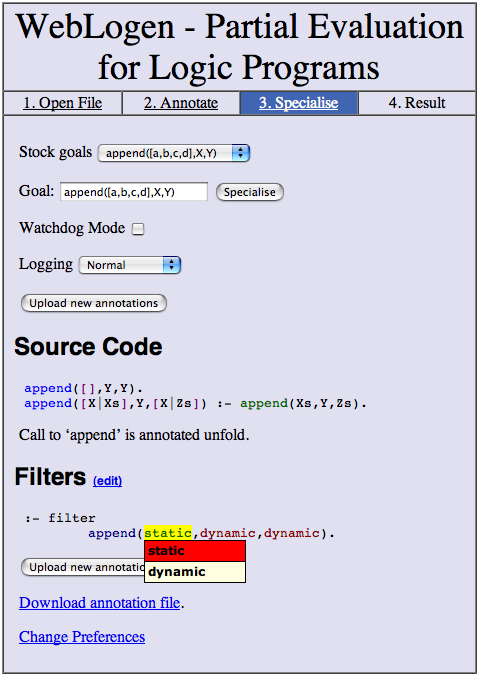
\includegraphics[width=3.5in]{Weblogen_screen}
\end{center}
%\caption{Converting source and annotation files to HTML}
%\protect\label{figure:ann2html}
%\end{figure}


\section{Presentation Outline}


\begin{enumerate}
\item Introduction
  \begin{itemize}
  \item Partial Evaluation for Prolog
 \item Offline Partial Evaluation
 \item The Cogen Approach
  \end{itemize}
 
 \item Design of the {\sc logen} system
  \begin{itemize}
    \item Overall layout
       \begin{itemize}
    \item Various files manipulated (source file, annotation file, gx files, specialised program)
     \item Various ingredients: the BTA, the cogen, the generating extensions, the annotation editing component
     \end{itemize}
    \item Structure of the annotations
    \item Architecture of the WebInterface/Server
           \begin{itemize}
    \item Various components
    \item Transforming the Prolog into XML and then using XSLT
    \item Using JavaScript to edit the annotations
    \item Security
    \end{itemize}
  \end{itemize}
  
 \item A simple Example, Complete walk-through
  \begin{itemize}
    \item Source program (e.g., regular expression matcher)
    \item Annotated source program
    \item Generating Extension
    \item Specialised Program
    \item Runtime Results
    \item Different Interfaces:
     \begin{itemize}
    \item The Command-Line Interface
    \item The Web Interface
    \end{itemize}
     
   \item Different ways to do the BTA:
     \begin{itemize}
    \item Simple BTA
    \item Automatic BTA
    \item How to edit manually
    \end{itemize}
  \end{itemize}
  
 \item Interpreters and Jones Optimality
  \begin{itemize}
    \item The plain vanilla self-interpreter
    \item  How to annotate it
    \item Show result \& Jones optimality
   \item Extending Plain vanilla:
  \begin{itemize}
    \item Debugging, Profiling, ...
  \end{itemize}
  \end{itemize}
    
    
 \item A More complicated Interpreter
   \begin{itemize}
    \item Show a more complicated interpreter:
    \item Illustrate binding-types (environment with partially static data),
     user-definable types
    \item Illustrate other annotations: call/rescall, use\_modules, operator declarations,..
   \end{itemize}
   
 \item Summary of other Applications
    \begin{itemize}
    \item Access Control
    \item Provably Correct Compilation
    \item Model Checking, ...
   \end{itemize}
   
 \item Advanced Features and New Developments
     \begin{itemize}
    \item Treatment of co-routines (when declarations)
    \item The Watchdog mode
    \item Semi-Online Annotations: semif, semicall,
      online unfold annotation, online binding-type
  \end{itemize}
  
\end{enumerate}


 \end{document}
 \end
 
